\section{Ausgabe von Drehmomentverläufen}

Damit die Drehmomente der Simulation ausgegeben werden können, soll die "Actuator Torque" Reihe in "Revolute Joint" eingecheckt werden.

\begin{figure}[!htbp]
	\centering
	\includegraphics[width=0.5\linewidth]{grafic/relovute_joint}
	\caption{Revolute Joint Simscape Block}
	\label{fig:simscape_revolute_joint}
\end{figure}

\begin{figure}[!htbp]
	\centering
	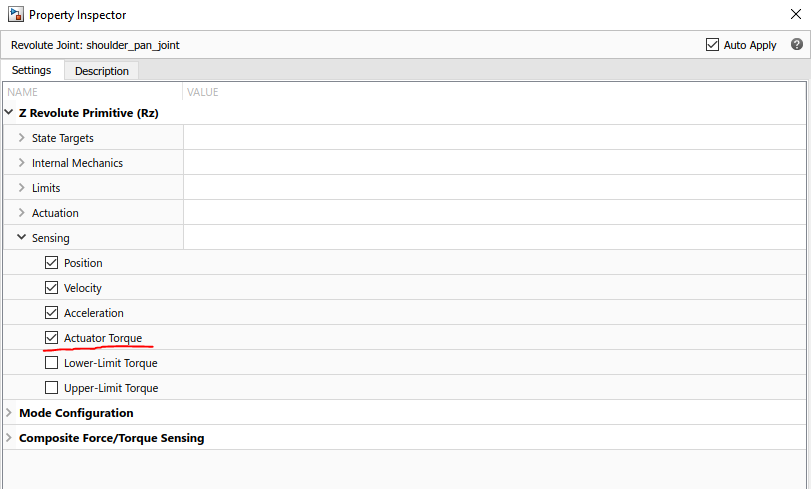
\includegraphics[width=0.5\linewidth]{grafic/actuator_torque}
	\caption{Actuator Torque Checkbox}
	\label{fig:simscape_relovute_joint_checkbox}
\end{figure}

Dann werden alle Ausgabe der Drehmomente von allen Gelenken mit BusCreator verbunden. Die Daten werden durch "Log Signals" Funktion der MATLAB eingelogt.

\begin{figure}[!htbp]
	\centering
	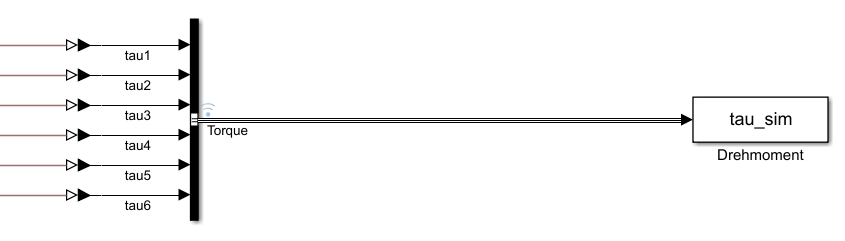
\includegraphics[width=1\linewidth]{grafic/torque_busline}
	\caption{Torque Bus Line and Log Sign}
	\label{fig:simulink_logging}
\end{figure}

Die Ergebnisse können in "Data Inspector" gesehen werden.

\begin{figure}[!htbp]
	\centering
	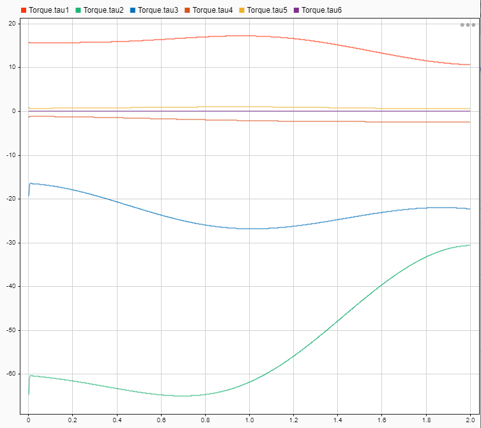
\includegraphics[width=1\linewidth]{grafic/Drehmomente}
	\caption{Ausgabe der Drehmomente}
	\label{fig:drehmomente_simulation}
\end{figure}

